



\lipsum[1-4]






\chapter{附录附录附录附录附录附录附录附录附录附录附录附录}


\begin{paracol}{2}

\footnote{测试文字}
\lipsum


\clearpage


\lipsum[3-4]


\end{paracol}


\footnote{测试文字}
\lipsum[1-2]


\lipsum[3-7]


\begin{paracol}{2}

\lipsum
\switchcolumnsloppy

\zhlipsum[1]

测试文字测试文字测试文字测试文字测试文字测试文字测试文字测试文字测试文字测试文字测试文字测试文字测试文字测试文字测试文字测试文字测试文字测试文字测试文字测试文字测试文字测试文字测试文字测试文字测试文字测试文字测试文字测试文字

\end{paracol}


\lipsum

\begin{Example}

\end{Example}

\begin{figure}
	\centering
	\begin{tikzpicture}[>=stealth, thick]
		\draw (0,0)--(2,0)--(2,1)--(0,1)--(0,0);
		\fill [pattern = north east lines] (-1,-.75) rectangle (3,-.5);
		\draw(-1,-.5)--(3,-.5);
		\draw (.5,-.25) circle (.225);
		\draw (1.5,-.25) circle (.225);
		\draw (.5,-.25) circle (.1);
		\draw (1.5,-.25) circle (.1);
		\draw[->, dashed](3,0.5)--(-2,0.5);
		\draw[very thick](0,.5)--(-2,0.5);
		\foreach \i in {-.4,-.8,-1.2,-1.6,-2}
		{
			\draw (\i,0.6)--(\i,.5);
		}
		\draw (-1,1)--(-1,1.1);
		\draw (-0.6,1)--(-0.6,1.1);
		\draw[-] (-1,1)--(-0.6,1);
		\node at (-0.8,1.35){$20$N};
	\end{tikzpicture}
	\caption{图中的虚线表示力的作用线}
\end{figure}


\chapterimage{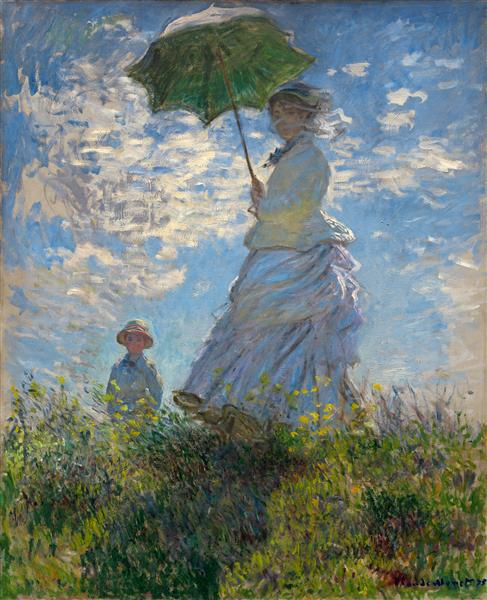
\includegraphics[height=\paperheight]{parasol.jpg}}
\chapter{附录1}
\zhlipsum[1]



\begin{figure}
	\centering
	\begin{tikzpicture}[>=stealth, thick]
		\draw (0,0)--(2,0)--(2,1)--(0,1)--(0,0);
		\fill [pattern = north east lines] (-1,-.75) rectangle (3,-.5);
		\draw(-1,-.5)--(3,-.5);
		\draw (.5,-.25) circle (.225);
		\draw (1.5,-.25) circle (.225);
		\draw (.5,-.25) circle (.1);
		\draw (1.5,-.25) circle (.1);
		\draw[->, dashed](3,0.5)--(-2,0.5);
		\draw[very thick](0,.5)--(-2,0.5);
		\foreach \i in {-.4,-.8,-1.2,-1.6,-2}
		{
			\draw (\i,0.6)--(\i,.5);
		}
		\draw (-1,1)--(-1,1.1);
		\draw (-0.6,1)--(-0.6,1.1);
		\draw[-] (-1,1)--(-0.6,1);
		\node at (-0.8,1.35){$20$N};
	\end{tikzpicture}
	\caption{图中的虚线表示力的作用线}
\end{figure}



\begin{Appendix}
\chapterimage{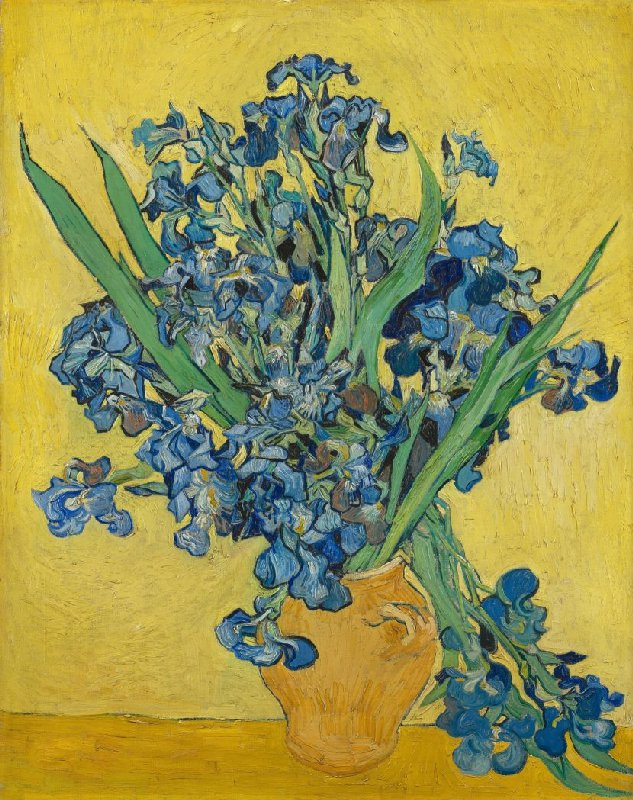
\includegraphics[height=\paperheight]{iris1.jpg}}
\chapter{附录2}
{\FontSizeSet[2.0]{16pt}
\lipsum
}

\begin{figure}
	\centering
	\begin{tikzpicture}[>=stealth, thick]
		\draw (0,0)--(2,0)--(2,1)--(0,1)--(0,0);
		\fill [pattern = north east lines] (-1,-.75) rectangle (3,-.5);
		\draw(-1,-.5)--(3,-.5);
		\draw (.5,-.25) circle (.225);
		\draw (1.5,-.25) circle (.225);
		\draw (.5,-.25) circle (.1);
		\draw (1.5,-.25) circle (.1);
		\draw[->, dashed](3,0.5)--(-2,0.5);
		\draw[very thick](0,.5)--(-2,0.5);
		\foreach \i in {-.4,-.8,-1.2,-1.6,-2}
		{
			\draw (\i,0.6)--(\i,.5);
		}
		\draw (-1,1)--(-1,1.1);
		\draw (-0.6,1)--(-0.6,1.1);
		\draw[-] (-1,1)--(-0.6,1);
		\node at (-0.8,1.35){$20$N};
	\end{tikzpicture}
	\caption{图中的虚线表示力的作用线}
\end{figure}



\section{附录测试}







	
\section{附录测试}



\begin{Topic}
\section{附录测试}

\subsubsection{看目录}

\subsubsection{看目录}

\subsubsection*{看目录}


\end{Topic}

\section{附录测试}


{\FontSizeSet[1.2]{14pt}\zhlipsum[1]}

	
\section{附录测试}
	
\end{Appendix}





\section{测量物体,包含长度测量}

\subsubsection{看目录}

\subsubsection{看目录}

\subsubsection*{看目录}

\begin{figure}
	\centering
	\begin{tikzpicture}[>=stealth, thick]
		\draw (0,0)--(2,0)--(2,1)--(0,1)--(0,0);
		\fill [pattern = north east lines] (-1,-.75) rectangle (3,-.5);
		\draw(-1,-.5)--(3,-.5);
		\draw (.5,-.25) circle (.225);
		\draw (1.5,-.25) circle (.225);
		\draw (.5,-.25) circle (.1);
		\draw (1.5,-.25) circle (.1);
		\draw[->, dashed](3,0.5)--(-2,0.5);
		\draw[very thick](0,.5)--(-2,0.5);
		\foreach \i in {-.4,-.8,-1.2,-1.6,-2}
		{
			\draw (\i,0.6)--(\i,.5);
		}
		\draw (-1,1)--(-1,1.1);
		\draw (-0.6,1)--(-0.6,1.1);
		\draw[-] (-1,1)--(-0.6,1);
		\node at (-0.8,1.35){$20$N};
	\end{tikzpicture}
	\caption{图中的虚线表示力的作用线}
\end{figure}


\part{丝柏树系列}





\chapterimage{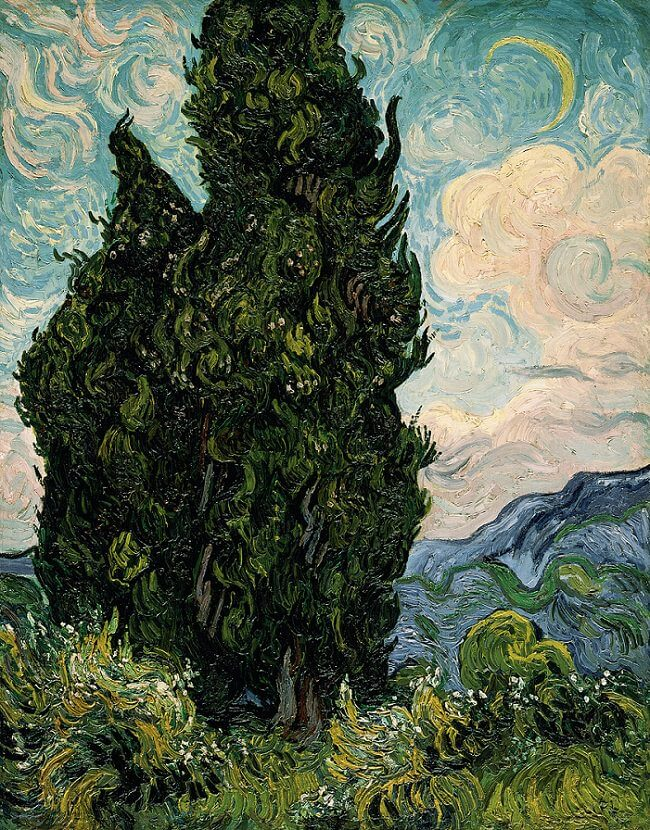
\includegraphics[height=\paperheight]{cypresses.jpg}}
\chapter{彩色计时器}

文森特·威廉·梵高(Vincent Willem van Gogh,1853年3月30日—1890年7月29日),荷兰后印象派画家。代表作有《星月夜》、自画像系列、向日葵系列等。

梵高出生于荷兰乡村津德尔特的一个新教牧师家庭,早年的他做过职员和商行经纪人,还当过矿区的传教士,最后他投身于绘画。他早期画风写实,受到荷兰传统绘画及法国写实主义画派的影响。1886年,他来到巴黎,结识印象派和新印象派画家,并接触到日本浮世绘的作品,视野的扩展使其画风巨变。1888年,来到法国南部小镇阿尔,创作《阿尔的吊桥》;同年与画家保罗·高更交往,但由于二人性格的冲突和观念的分歧,合作很快便告失败。此后,梵高的疯病(有人记载是“癫痫病”)时常发作,但神志清醒时他仍然坚持作画。1889年创作《星月夜》。1890年7月,梵高在精神错乱中开枪自杀(一说,两个年轻人不小心走火开枪击中),年仅37岁。

梵高是表现主义的先驱,并深深影响了二十世纪艺术,尤其是野兽派与德国表现主义。\footnote{本章封面画为荷兰画家文森特·梵高的《柏树》。}







\section{测量物体,包含长度测量}

\footnote{测试文字}






\chapterimage{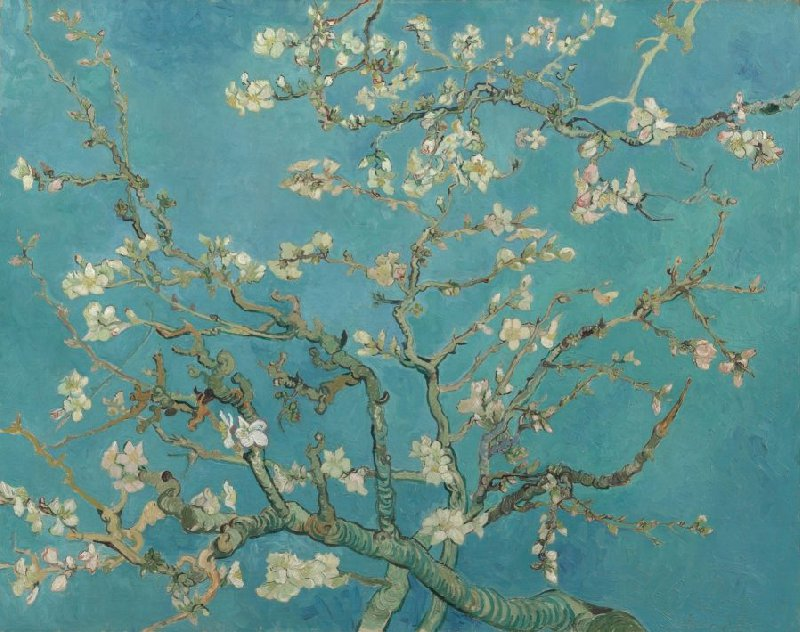
\includegraphics[height=\paperheight]{blossom.jpg}}
\chaptersaying{文王拘而演周易,仲尼厄而作春秋。}
\chapter{测量}

\footnote{看看我}\zhlipsum

\section{测量物体,包含长度测量}

\begin{Example}
	测试文字测试文字
\end{Example}




\section{测量物体,包含长度测量}

\section{测量物体,包含长度测量}
\footnote{测试文字}\lipsum








\begin{Project}

\section{测量物体,包含长度测量}

\begin{Point*}
	学习完这一单元,你应当能够: 识别国际单位制(SI)中的基本量; 正确称呼国际单位制中最常用的词头; 利用链环变换法改变单位(这里是对于长度、面积和体积); 说明米是如何用真空中光速来定义的。
	\tcblower
	\tcbsubtitle{本节重点\footnote{脚注}}
	物理学是以物理量的测量为基础的。一些物理量被选作基本物理量; 每一种基本物理量都已经通过一种标准来定义并给定测量的单位。另一些物理量是用这些基本物理量和它们的标准及单位来定义。

\end{Point*}

测试文字测试文字测试文字测试文字测试文字测试文字测试文字测试文字测试文字测试文字测试文字测试文字测试文字测试文字测试文字测试文字测试文字测试文字测试文字测试文字测试文字测试文字测试文字测试文字测试文字测试文字




\begin{paracol}{2}
	\subsection{什么是物理学?}

	
	科学和工程学建立在测量和比较的基础上。因此,我们就需要关于如何测量和比较物体的规则,并且我们还需要通过实验来建立这种测量和比较的单位。物理学(以及工程学)的一个目的就是设计和实施这些实验。
	\marginpar{测试文字测试文字测试文字测试文字测试文字测试文字}
	
	例如,物理学家们尽力开发极其准确的时钟从而使任何时间或时间间隔都可以精确地确定和比较。你们可能要问,这样的准确度是否真正需要,或者是否值得花这么大的精力。这里给出一个是否值得的例子:如果没有极其准确的时钟的话,那么现在全世界范围的航行必不可少的全球定位系统(GPS)就会变得毫无意义。
	\RelaInfo*{测试文字测试文字测试文字测试文字测试文字测试文字测试文字测试文字测试文字测试文字测试文字测试文字\footnote{看看我}
	}
	
	\subsection{测量物体}
	\NoteArea
	
	\subsubsection{测试文字}
	
	我们通过学习怎样测量物理学中的量来学习物理学。这些物理量包括长度、时间、质量、温度、压强和电流。\footnote{看看我}
	
	我们通过和一个标准相比较,用它们各自的单位来量度各个
	
	
	
	
	
\end{paracol}

\subsection{力的三要素}


\subsubsection{测试文字}

力是有大小的.我们在初中学过,力的大小可以用测力计来测量.在国际单位制中力的单位是\textbf{牛顿},简称牛,国际符号是N,日常生活和生产中常用的力的单位是千克力,牛顿和千克力的关系是:1千克力$=9.8$牛.

力不但有大小,而且有方向.物体受到的重力是竖直向下的,物体在液体中受到的浮力是竖直向上的,力的方向不同,它的作用效果也不同.用力拉弹簧,弹簧就伸长;用反方向的力压弹簧,弹簧就缩短.作用在运动物体上的力,如果方向与运动方向相同,将加快物体的运动;如果方向与运动方向相反,将阻碍物体的运动.可见,要把一个力完全表达出来,除了说明力的大小外,还要指明力的方向.

\begin{wrapfigure}[6]{r}{6cm}
	\vspace*{-1.5em}
	\centering
	\begin{tikzpicture}[>=stealth, thick]
		\draw (0,0)--(2,0)--(2,1)--(0,1)--(0,0);
		\fill [pattern = north east lines] (-1,-.75) rectangle (3,-.5);
		\draw(-1,-.5)--(3,-.5);
		\draw (.5,-.25) circle (.225);
		\draw (1.5,-.25) circle (.225);
		\draw (.5,-.25) circle (.1);
		\draw (1.5,-.25) circle (.1);
		\draw[->, dashed](3,0.5)--(-2,0.5);
		\draw[very thick](0,.5)--(-2,0.5);
		\foreach \i in {-.4,-.8,-1.2,-1.6,-2}
		{
			\draw (\i,0.6)--(\i,.5);
		}
		\draw (-1,1)--(-1,1.1);
		\draw (-0.6,1)--(-0.6,1.1);
		\draw[-] (-1,1)--(-0.6,1);
		\node at (-0.8,1.35){$20$N};
	\end{tikzpicture}
	\caption{图中的虚线表示力的作用线}
\end{wrapfigure}
为了直观地说明力的作用,常常用一根带箭头的线段来表示力.线段是按一定比
例(标度)画出的,它的长短表示力的大小,它的指向表示力的方向,箭头或箭尾表示力的作用点,箭头所沿的直线叫做力的作用线.这种表示力的方法,叫做\textbf{力的图示}.图1.1中表示的是作用在小车上的$100$N的力.

\subsection{力的分类\protect\footnote{测试文字}}

我们从初中开始学习物理以来,见过的力的名称已经相当多了.各种力可以用不同的方法来分类.一种是根据力的性质来分类的,如重力、弹力、摩擦力、分子力、电磁力等;另一种是根据力的效果来分类的,如拉力、压力、支持力、动力、阻力等等.拉力、压力、支持力实际上都是弹力,只是效果不同.不论是什么性质的力,只要效果是加快物体的运动,就可以叫它为动力;效果是阻碍物体的运动,就可以叫它为阻力.今后我们还会遇到根据效果来命名的力的名称.

从力的性质来看,力学中经常遇到的有重力、弹力、摩擦力.下面几节就分别介绍这三种力.


\begin{Example}
	测试文字测试文字测试文字测试文字测试文字测试文字测试文字测试文字测试文字测试文字测试文字测试文字测试文字测试文字测试文字测试文字测试文字测试文字测试文字测试文字测试文字测试文字测试文字测试文字测试文字测试文字测试文字测试文字测试文字测试文字测试文字测试文字测试文字测试文字测试文字测试文字测试文字测试文字测试文字测试文字测试文字
	\begin{flalign}
		\Psi=\int_\Omega\left[f\left(\phi\right)+\kappa\left|\nabla\phi\right|^2\right]{\rm d}V
	\end{flalign}
\end{Example}

\begin{Example}
	测试文字测试文字\footnote{看看我}
\end{Example}


\subsection{测试文字}
\subsection*{测试文字}
\zhlipsum[1]


\makeatletter



\makeatother

\begin{multicols}{2}
\Basis

\Complex
\end{multicols}

\zhlipsum[1]

















\clearpage

\Improve
\begin{QuestionItem}[2]
	\item 关于行星运动的规律,下列说法符合史实的是
	\choice{开普勒在牛顿定律的基础上,导出了行星运动的规律}{开普勒在天文观测数据的基础上,总结出了行星运动的规律}{开普勒总结出了行星运动的规律,找出了行星按照这些规律运动的原因}{开普勒总结出了行星运动的规律,发现了万有引力定律}
	\item 火星和木星沿各自的椭圆轨道绕太 阳运行,根据开普勒行星运动定律可知
	\choice{太阳位于木星运行轨道的中心}{火星和木星绕太阳运行速度的大小始终相等}{火星与木星公转周期之比的平方等于它们轨道半长轴之比的立方}{相同时间内,火星与太阳连线扫过的面积等于木星与太阳连线扫过的面积}
	\item 为了探测引力波,“天琴计划” 预计发射地球卫星P,其轨道半径约为地球半径的16倍;另一地球卫星Q的轨道半径约为地球半径的4倍。P与Q的周期之比约为
	\choice{2∶1}{4∶1}{8∶1}{16∶1}
	\item 测试文字测试文字测试文字测试文字测试文字测试文字测试文字测试文字测试文字测试文字测试文字测试文字测试文字测试文字测试文字测试文字测试文字测试文字测试文字测试文字测试文字测试文字测试文字测试文字测试文字测试文字测试文字测试文字测试文字测试文字测试文字测试文字测试文字测试文字测试文字测试文字测试文字测试文字测试文字测试文字测试文字测试文字测试文字测试文字测试文字测试文字测试文字测试文字
	\item 测试文字测试文字测试文字测试文字测试文字测试文字测试文字测试文字测试文字测试文字测试文字测试文字测试文字测试文字测试文字测试文字测试文字测试文字测试文字测试文字测试文字测试文字测试文字测试文字测试文字测试文字测试文字测试文字测试文字测试文字测试文字测试文字测试文字测试文字测试文字测试文字测试文字测试文字测试文字测试文字测试文字测试文字测试文字测试文字测试文字测试文字测试文字测试文字
	\item 测试文字测试文字测试文字测试文字测试文字测试文字测试文字测试文字测试文字测试文字测试文字测试文字测试文字测试文字测试文字测试文字测试文字测试文字测试文字测试文字测试文字测试文字测试文字测试文字测试文字测试文字测试文字测试文字测试文字测试文字测试文字测试文字测试文字测试文字测试文字测试文字测试文字测试文字测试文字测试文字测试文字测试文字测试文字测试文字测试文字测试文字测试文字测试文字
	\item 测试文字测试文字测试文字测试文字测试文字测试文字测试文字测试文字测试文字测试文字测试文字测试文字测试文字测试文字测试文字测试文字测试文字测试文字测试文字测试文字测试文字测试文字测试文字测试文字测试文字测试文字测试文字测试文字测试文字测试文字测试文字测试文字测试文字测试文字测试文字测试文字测试文字测试文字测试文字测试文字测试文字测试文字测试文字测试文字测试文字测试文字测试文字测试文字
	\item 测试文字测试文字测试文字测试文字测试文字测试文字测试文字测试文字测试文字测试文字测试文字测试文字测试文字测试文字测试文字测试文字测试文字测试文字测试文字测试文字测试文字测试文字测试文字测试文字测试文字测试文字测试文字测试文字测试文字测试文字测试文字测试文字测试文字测试文字测试文字测试文字测试文字测试文字测试文字测试文字测试文字测试文字测试文字测试文字测试文字测试文字测试文字测试文字
	\item 测试文字测试文字测试文字测试文字测试文字测试文字测试文字测试文字测试文字测试文字测试文字测试文字测试文字测试文字测试文字测试文字测试文字测试文字测试文字测试文字测试文字测试文字测试文字测试文字测试文字测试文字测试文字测试文字测试文字测试文字测试文字测试文字测试文字测试文字测试文字测试文字测试文字测试文字测试文字测试文字测试文字测试文字测试文字测试文字测试文字测试文字测试文字测试文字
	\item 测试文字测试文字测试文字测试文字测试文字测试文字测试文字测试文字测试文字测试文字测试文字测试文字测试文字测试文字测试文字测试文字测试文字测试文字测试文字测试文字测试文字测试文字测试文字测试文字测试文字测试文字测试文字测试文字测试文字测试文字测试文字测试文字测试文字测试文字测试文字测试文字测试文字测试文字测试文字测试文字测试文字测试文字测试文字测试文字测试文字测试文字测试文字测试文字
	\item 测试文字测试文字测试文字测试文字测试文字测试文字测试文字测试文字测试文字测试文字测试文字测试文字测试文字测试文字测试文字测试文字测试文字测试文字测试文字测试文字测试文字测试文字测试文字测试文字测试文字测试文字测试文字测试文字测试文字测试文字测试文字测试文字测试文字测试文字测试文字测试文字测试文字测试文字测试文字测试文字测试文字测试文字测试文字测试文字测试文字测试文字测试文字测试文字
	\item 测试文字测试文字测试文字测试文字测试文字测试文字测试文字测试文字测试文字测试文字测试文字测试文字测试文字测试文字测试文字测试文字测试文字测试文字测试文字测试文字测试文字测试文字测试文字测试文字测试文字测试文字测试文字测试文字测试文字测试文字测试文字测试文字测试文字测试文字测试文字测试文字测试文字测试文字测试文字测试文字测试文字测试文字测试文字测试文字测试文字测试文字测试文字测试文字
	\item 测试文字测试文字测试文字测试文字测试文字测试文字测试文字测试文字测试文字测试文字测试文字测试文字测试文字测试文字测试文字测试文字测试文字测试文字测试文字测试文字测试文字测试文字测试文字测试文字测试文字测试文字测试文字测试文字测试文字测试文字测试文字测试文字测试文字测试文字测试文字测试文字测试文字测试文字测试文字测试文字测试文字测试文字测试文字测试文字测试文字测试文字测试文字测试文字
	\item 测试文字测试文字测试文字测试文字测试文字测试文字测试文字测试文字测试文字测试文字测试文字测试文字测试文字测试文字测试文字测试文字测试文字测试文字测试文字测试文字测试文字测试文字测试文字测试文字测试文字测试文字测试文字测试文字测试文字测试文字测试文字测试文字测试文字测试文字测试文字测试文字测试文字测试文字测试文字测试文字测试文字测试文字测试文字测试文字测试文字测试文字测试文字测试文字
	\item 测试文字测试文字测试文字测试文字测试文字测试文字测试文字测试文字测试文字测试文字测试文字测试文字测试文字测试文字测试文字测试文字测试文字测试文字测试文字测试文字测试文字测试文字测试文字测试文字测试文字测试文字测试文字测试文字测试文字测试文字测试文字测试文字测试文字测试文字测试文字测试文字测试文字测试文字测试文字测试文字测试文字测试文字测试文字测试文字测试文字测试文字测试文字测试文字
	\item 测试文字测试文字测试文字测试文字测试文字测试文字测试文字测试文字测试文字测试文字测试文字测试文字测试文字测试文字测试文字测试文字测试文字测试文字测试文字测试文字测试文字测试文字测试文字测试文字测试文字测试文字测试文字测试文字测试文字测试文字测试文字测试文字测试文字测试文字测试文字测试文字测试文字测试文字测试文字测试文字测试文字测试文字测试文字测试文字测试文字测试文字测试文字测试文字
\end{QuestionItem}


\Thinking
	\begin{QuestionItem}
		\item 测试文字测试文字测试文字测试文字测试文字测试文字测试文字测试文字测试文字测试文字测试文字测试文字测试文字测试文字测试文字测试文字测试文字测试文字测试文字测试文字测试文字测试文字测试文字测试文字测试文字测试文字测试文字测试文字测试文字测试文字测试文字测试文字测试文字测试文字测试文字测试文字测试文字测试文字测试文字测试文字测试文字测试文字测试文字测试文字测试文字测试文字测试文字测试文字
		\item 测试文字测试文字测试文字测试文字测试文字测试文字测试文字测试文字测试文字测试文字测试文字测试文字测试文字测试文字测试文字测试文字测试文字测试文字测试文字测试文字测试文字测试文字测试文字测试文字测试文字测试文字测试文字测试文字测试文字测试文字测试文字测试文字测试文字测试文字测试文字测试文字测试文字测试文字测试文字测试文字测试文字测试文字测试文字测试文字测试文字测试文字测试文字测试文字
		\item 测试文字测试文字测试文字测试文字测试文字测试文字测试文字测试文字测试文字测试文字测试文字测试文字测试文字测试文字测试文字测试文字测试文字测试文字测试文字测试文字测试文字测试文字测试文字测试文字测试文字测试文字测试文字测试文字测试文字测试文字测试文字测试文字测试文字测试文字测试文字测试文字测试文字测试文字测试文字测试文字测试文字测试文字测试文字测试文字测试文字测试文字测试文字测试文字
		\item 测试文字测试文字测试文字测试文字测试文字测试文字测试文字测试文字测试文字测试文字测试文字测试文字测试文字测试文字测试文字测试文字测试文字测试文字测试文字测试文字测试文字测试文字测试文字测试文字测试文字测试文字测试文字测试文字测试文字测试文字测试文字测试文字测试文字测试文字测试文字测试文字测试文字测试文字测试文字测试文字测试文字测试文字测试文字测试文字测试文字测试文字测试文字测试文字
	\end{QuestionItem}


\begin{Definition}[测试文字\footnote{测试脚注测试脚注测试脚注测试脚注测试脚注测试脚注测试脚注测试脚注测试脚注测试脚注测试脚注测试脚注测试脚注测试脚注测试脚注测试脚注测试脚注}]
	测试文字\footnote{脚注}
	\begin{flalign}
		\Psi=\int_\Omega\left[f\left(\phi\right)+\kappa\left|\nabla\phi\right|^2\right]{\rm d}V
	\end{flalign}
\end{Definition}

\begin{Lemma}
	测试文字
\end{Lemma}

\begin{Theorem}[测试文字测试文字测试文字测试文字测试文字测试文字测试文字测试文字测试文字测试文字测试文字测试文字测试文字]
	测试文字
\end{Theorem}

\begin{Axiom}[测试文字][测试文字]
	测试文字
\end{Axiom}


\begin{Proposition}
	测试文字
\end{Proposition}


\begin{Corollary}
	\lipsum[1]
\end{Corollary}

\begin{Lemma}[测试文字\footnote{脚注}]
	测试文字\footnote{看看我}
\end{Lemma}


\begin{Lemma*}[测试文字测试文字]
	测试文字测试文字测试文字测试文字测试文字测试文字测试文字测试文字测试文字测试文字
	
	测试文字测试文字测试文字测试文字测试文字测试文字测试文字测试文字测试文字测试文字
	\zhlipsum
	测试文字测试文字测试文字测试文字测试文字测试文字测试文字测试文字测试文字测试文字测试文字测试文字
	\tcblower
	\tcbsubtitle{测试文字}
	\zhlipsum[2]
	\tcbsubtitle{副标题}
	\zhlipsum[2]\footnote{看看我}
\end{Lemma*}



\begin{linenumbers}
\lipsum[1]
\end{linenumbers}





\begin{multicols}{3}
\LongHeading{测试文字\footnote{看看我}}
测试文字测试文字测试文字测试文字测试文字测试文字测试文字测试文字测试文字测试文字测试文字测试文字测试文字测试文字测试文字
\LongHeading{测试文字}
测试文字测试文字测试文字测试文字测试文字测试文字测试文字测试文字测试文字测试文字测试文字测试文字测试文字测试文字测试文字
\LongHeading{测试文字}
测试文字测试文字测试文字测试文字测试文字测试文字测试文字测试文字测试文字测试文字测试文字测试文字测试文字测试文字测试文字
\end{multicols}




\Listening

\Reading

\Writing

\Speaking

\AdjustiveHeading{测试文字\footnote{看看我}}

\lipsum[1][1-5]

\begin{UnnumberedItem}[3]

\item test
\item test
\item test
\item test
\item test
\item test
\item test
\item test
\item test
\end{UnnumberedItem}

\begin{NumberedItem}
	\item 测试文字
	\item test
	\item testqjply\footnote{看看我}
\end{NumberedItem}



\begin{Proof}
	\lipsum[1]\footnote{看看我}
	\tcblower
	\lipsum
\end{Proof}

\begin{Block}%[测试文字]
	\lipsum[1]
	\tcblower
	\footnote{测试文字}\lipsum
\end{Block}


\begin{Check}
	\lipsum[1-2]
	\tcbline
	\lipsum[1-2]
\end{Check}

\begin{Warning}
	\lipsum[2]
	\tcbsubtitle{测试文字}
	\tcblower
	\tcbsubtitle{测试文字}
	cswz
\end{Warning}



\begin{Comprehension}[测试文字\footnote{脚注}]
		\lipsum
	\begin{NumberedItem}
		\item 测试文字
	\end{NumberedItem}
\end{Comprehension}



\Remark{\zhlipsum[1]%
\tcblower%
\zhlipsum[2]}









\begin{PythonBox}[神经网络]
import pytorch as pt
import numpy as np
import pandas as pd
import pytorch as pt
import numpy as np
import pandas as pd
import pytorch as pt
import numpy as np
import pytorch as pt
import numpy as np
import pandas as pd
import pytorch as pt
import numpy as np
import pandas as pd
import pandas as pd
import pytorch as pt
import numpy as np
import pandas as pd
import pytorch as pt
import numpy as np
import pandas as pd
\end{PythonBox}














\Homework
\Basis
\zhlipsum[1]
\Complex
\zhlipsum[2]




\begin{figure}
	\centering
\begin{tikzpicture}[>=stealth, thick]
	\draw (0,0)--(2,0)--(2,1)--(0,1)--(0,0);
	\fill [pattern = north east lines] (-1,-.75) rectangle (3,-.5);
	\draw(-1,-.5)--(3,-.5);
	\draw (.5,-.25) circle (.225);
	\draw (1.5,-.25) circle (.225);
	\draw (.5,-.25) circle (.1);
	\draw (1.5,-.25) circle (.1);
	\draw[->, dashed](3,0.5)--(-2,0.5);
	\draw[very thick](0,.5)--(-2,0.5);
	\foreach \i in {-.4,-.8,-1.2,-1.6,-2}
	{
		\draw (\i,0.6)--(\i,.5);
	}
	\draw (-1,1)--(-1,1.1);
	\draw (-0.6,1)--(-0.6,1.1);
	\draw[-] (-1,1)--(-0.6,1);
	\node at (-0.8,1.35){$20$N};
\end{tikzpicture}
\caption{图中的虚线表示力的作用线}
\end{figure}




\end{Project}









\section{测试文字}

\makeatletter
\@SubsectionStarStyle{测试文字}{测试文字}
\makeatother
\subsubsection{测试文字}
\lipsum



\subsection{测试文字}
\subsubsection{测试文字}


\subsection{测试文字}
\subsubsection{测试文字}
\subsubsection{测试文字}
\subsubsection{测试文字}

\begin{Example}
	测试文字测试文字测试文字测试文字测试文字测试文字测试文字测试文字测试文字测试文字测试文字测试文字测试文字测试文字测试文字测试文字测试文字测试文字测试文字测试文字测试文字测试文字测试文字测试文字测试文字测试文字测试文字测试文字测试文字测试文字测试文字测试文字测试文字测试文字测试文字测试文字测试文字测试文字测试文字测试文字测试文字
	\begin{flalign}
		\Psi=\int_\Omega\left[f\left(\phi\right)+\kappa\left|\nabla\phi\right|^2\right]{\rm d}V
	\end{flalign}
\end{Example}




\Improve
\begin{QuestionItem}[2]
	\item test$\Psi=\int_\Omega\left[f\left(\phi\right)+\kappa\left|\nabla\phi\right|^2\right]{\rm d}V$
	\item test
	$$\Psi=\int_\Omega\left[f\left(\phi\right)+\kappa\left|\nabla\phi\right|^2\right]{\rm d}V$$
	\item test
	\item test
	\item test
	\item test
	\item test
	\item test
\end{QuestionItem}


\Thinking
\begin{QuestionItem}
	\item 测试文字
	\item 测试文字
	\item 测试文字
	\item 测试文字
\end{QuestionItem}








\chapterimage{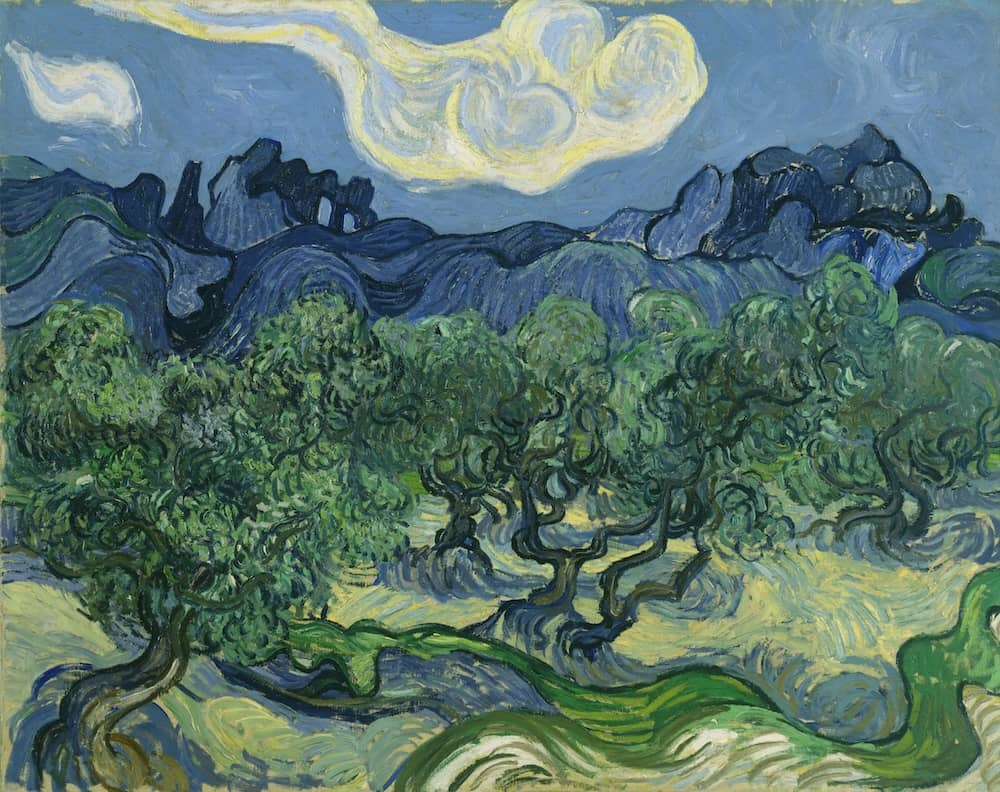
\includegraphics[height=\paperheight]{olive.jpg}}
\chapter{测试文字}

\zhlipsum



\begin{Appendix*}
	

\chapterimage{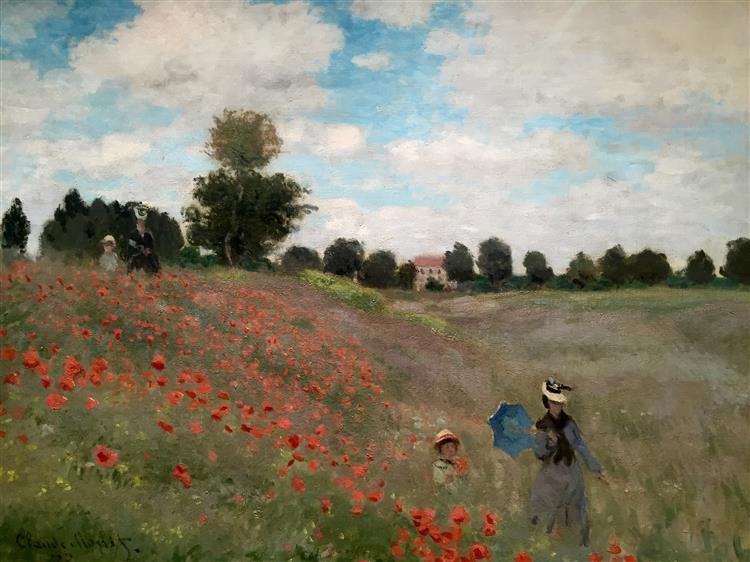
\includegraphics[height=\paperheight]{poppies.jpg}}
\chapter{测试计数器}
	
\section{附录测试}

\section{附录测试}

\end{Appendix*}



	
	
\chapterimage{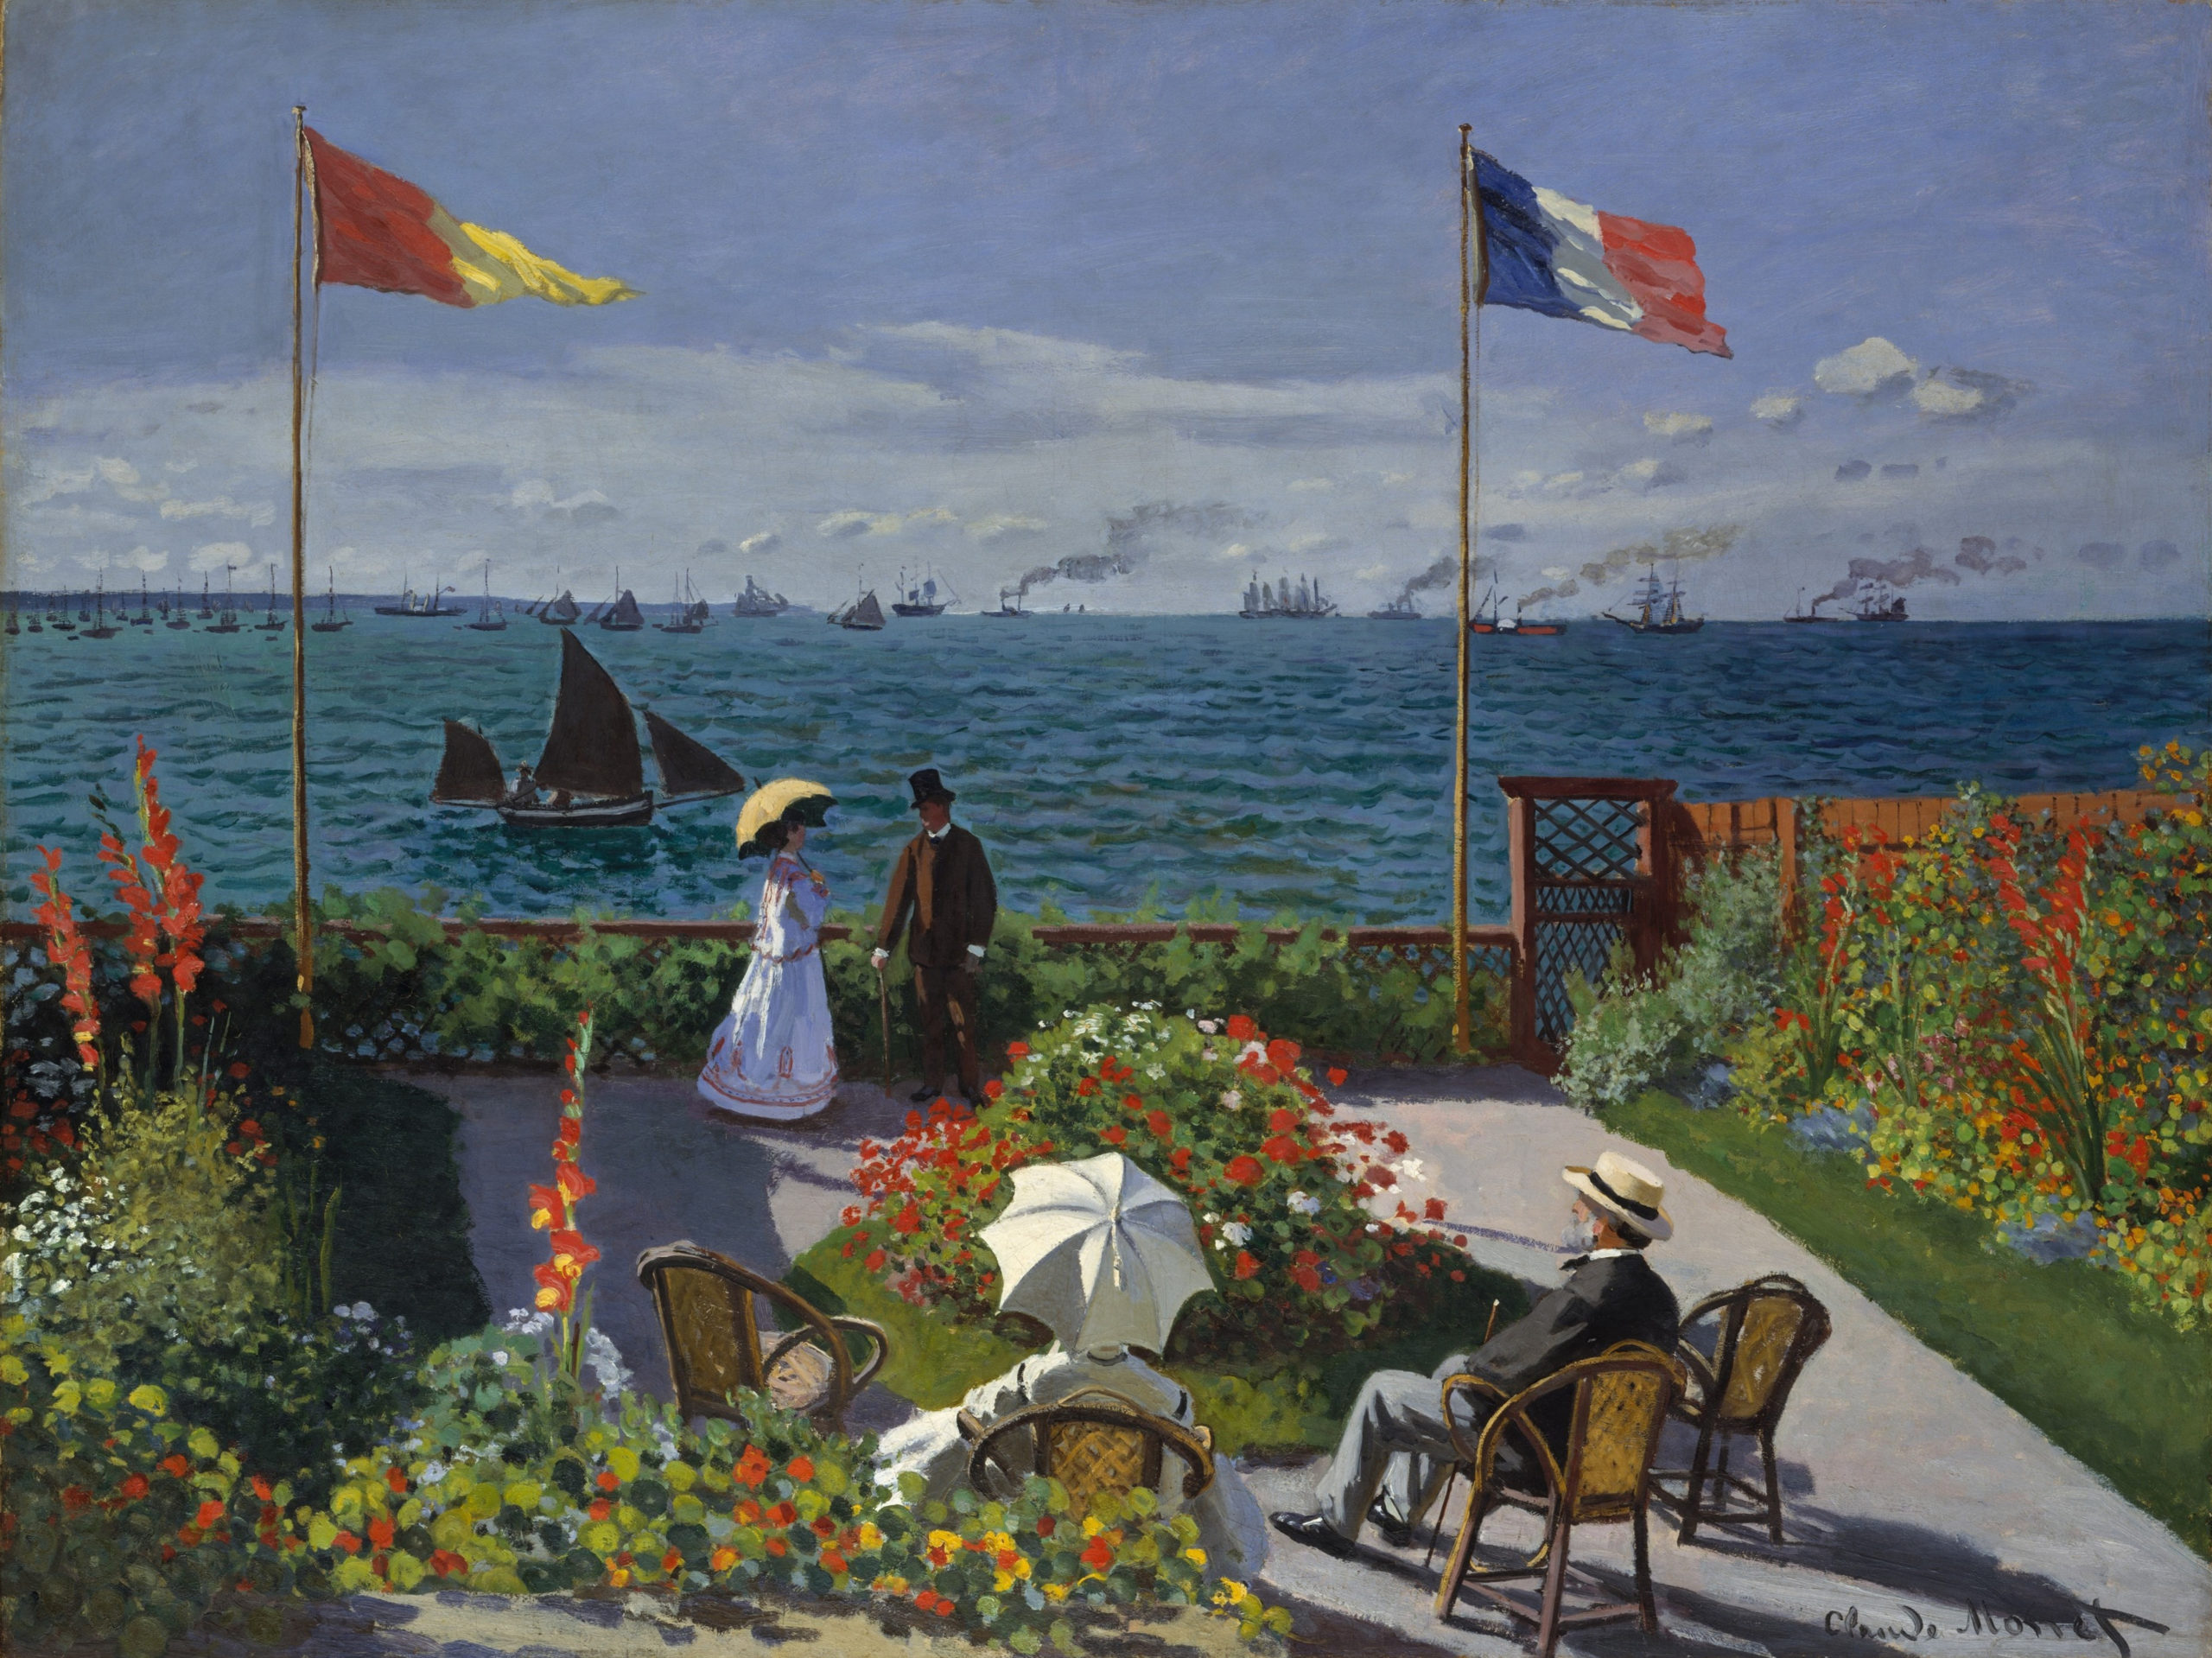
\includegraphics[height=\paperheight]{garden.jpg}}
\chapter{测试计数器}
奥斯卡-克劳德·莫奈(法文:Oscar-Claude Monet,1840年11月14日——1926年12月5日),法国画家,被誉为“印象派领导者”,印象派代表人物和创始人之一。

莫奈是法国最重要的画家之一,印象派的理论和实践大部分都有他的推广。莫奈擅长光与影的实验与表现技法。他最重要的风格是改变了阴影和轮廓线的画法,在莫奈的画作中看不到非常明确的阴影,也看不到突显或平涂式的轮廓线。光和影的色彩描绘是莫奈绘画的最大特色。

从印象主义的产生、发展看,创始人并非莫奈,但真正完全实现印象主义理念和技法、并且一以贯之的当推莫奈。是他将毕生精力献给了对西方画界产生了重要影响的印象主义,是以他为首的一批艺术家的不懈努力,突破了此前学院派的保守思想,极大地冲击了19世纪后半叶占据西方画坛统治地位的官方艺术,从而为掀开西方现代绘画史新的一页,作出了重要贡献。为后人留下了宝贵的艺术财富。应该说莫奈是印象派画家中最先获得成功的人,尽管后来的野兽派、立体派、超现实主义等艺术流派,并未遵循印象派创立的一些原则,但创立这些流派的艺术家,都从印象派那里汲取过营养。\footnote{本章封面画为法国画家克劳德·莫奈的《圣阿德雷斯的阳台》。}


\section{附录测试}

\subsection{Look and Read}

\section{附录测试}
	




\chapterimage{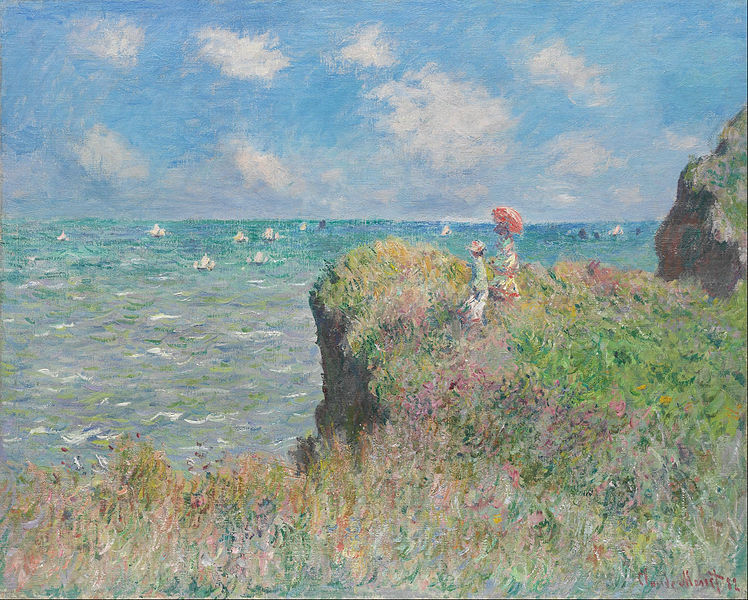
\includegraphics[height=\paperheight]{clifftop.jpg}}
\chapter{中间}




\chapterimage{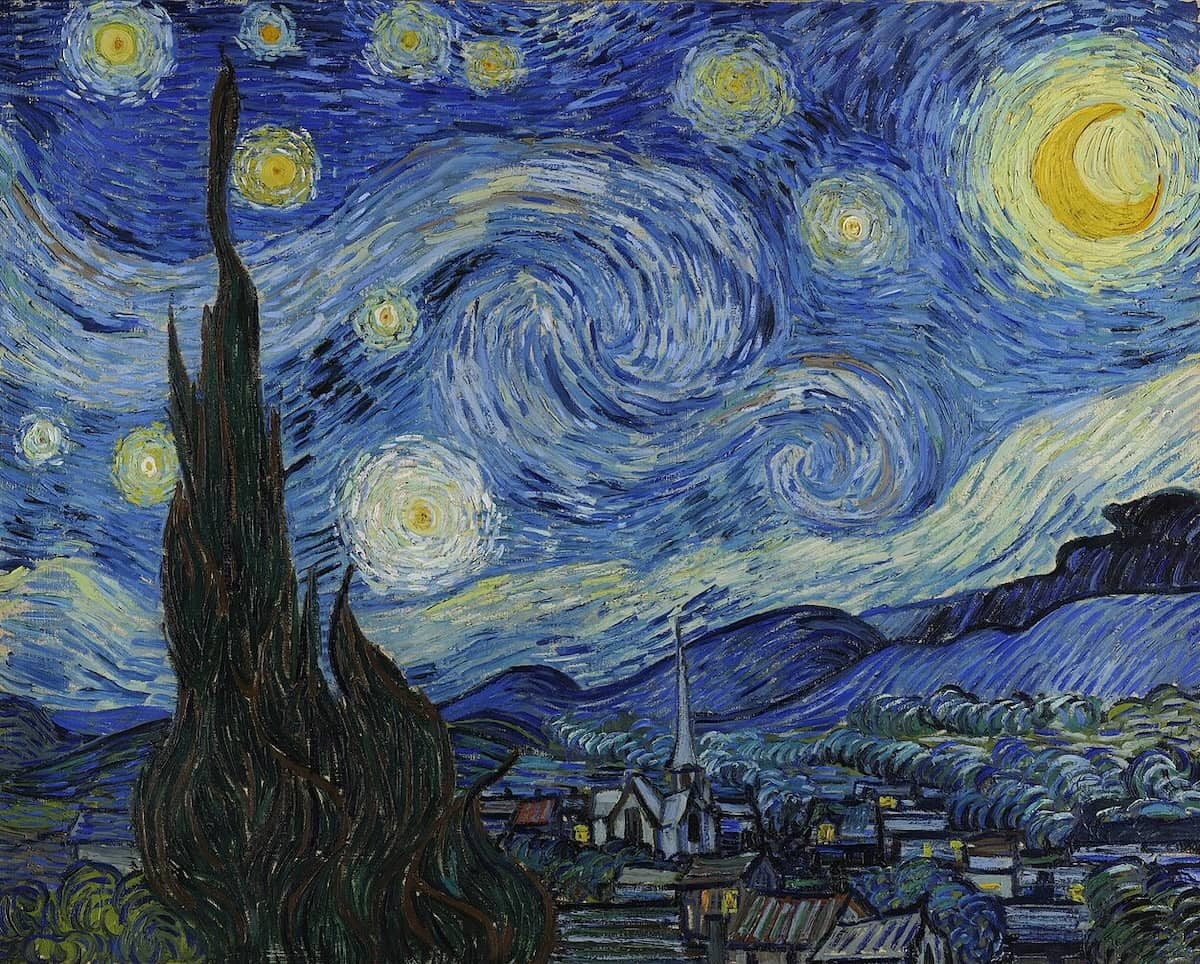
\includegraphics[height=\paperheight]{starry.jpg}}
\chapter{测试}
	



\begin{figure}
	\centering
	\begin{tikzpicture}[>=stealth, thick]
		\draw (0,0)--(2,0)--(2,1)--(0,1)--(0,0);
		\fill [pattern = north east lines] (-1,-.75) rectangle (3,-.5);
		\draw(-1,-.5)--(3,-.5);
		\draw (.5,-.25) circle (.225);
		\draw (1.5,-.25) circle (.225);
		\draw (.5,-.25) circle (.1);
		\draw (1.5,-.25) circle (.1);
		\draw[->, dashed](3,0.5)--(-2,0.5);
		\draw[very thick](0,.5)--(-2,0.5);
		\foreach \i in {-.4,-.8,-1.2,-1.6,-2}
		{
			\draw (\i,0.6)--(\i,.5);
		}
		\draw (-1,1)--(-1,1.1);
		\draw (-0.6,1)--(-0.6,1.1);
		\draw[-] (-1,1)--(-0.6,1);
		\node at (-0.8,1.35){$20$N};
	\end{tikzpicture}
	\caption{图中的虚线表示力的作用线}
\end{figure}


	


